\documentclass[12pt,a4paper]{article}
\usepackage[utf8]{inputenc}
\usepackage[dvipsnames]{xcolor}
\usepackage{dsfont}
\usepackage[nohead]{geometry}
\usepackage{amssymb}
\usepackage{amsfonts}
\usepackage{amsmath}
\usepackage[onehalfspacing]{setspace}
\usepackage[bottom]{footmisc}
\usepackage{endnotes}
\usepackage{graphicx}
\usepackage{rotating}
\usepackage{enumerate}
\usepackage{hyperref}
\usepackage{subcaption}
\usepackage[thmmarks,amsmath,amsthm,hyperref]{ntheorem}
\usepackage{enumitem}
\usepackage[shortlabels]{enumitem}

\theoremstyle{break}

\makeatletter
\def\@biblabel#1{\hspace*{-\labelsep}}
\makeatother
\geometry{left=1in,right=1in,top=1.00in,bottom=1.0in}
\newdimen\dummy
\dummy=\oddsidemargin
\addtolength{\dummy}{72pt}
\marginparwidth=.5\dummy
\marginparsep=.1\dummy

\begin{document}

    \noindent
    \textsc{Environmental Economics Lab}  \hspace{\stretch{1}}
    \textsc{1\textsuperscript{st} Semester 2024}

    \noindent
    \textsc{Prof. Pedro Henrique Chaves Maia}  \hspace{\stretch{1}}
    \textsc{FGV EPGE}

    \noindent
    \textsc{TA: Vinícius Hector}
    
    \bigskip
    \hrule

    \begin{center}
        \textsc{Problem Set \#1 - Solutions}
    \end{center}
    \hrule

\bigskip
\bigskip

\indent O código em anexo é uma sugestão de solução para a lista. Note que não há somente uma resposta correta. Desde que os passos sejam bem justificados, problemas práticos admitem várias soluções. Ao longo do código discutimos como solucioná-los até chegar nos resultados finais.\\
\indent Certifique-se de que todos os arquivos estão na pasta correta e também confira se todos os pacotes estão instalados.\\

\textbf{Item 1}\\
\ident Ao executar o notebook com a solução proposta, encontramos que as áreas (ou subprefeituras) que mais geraram IPTU em 2023 foram:\\

\begin{figure}[htbp]
  \centering
  % Adjust the widths and the figure names to suit your document
  \begin{subfigure}[b]{0.32\textwidth}
    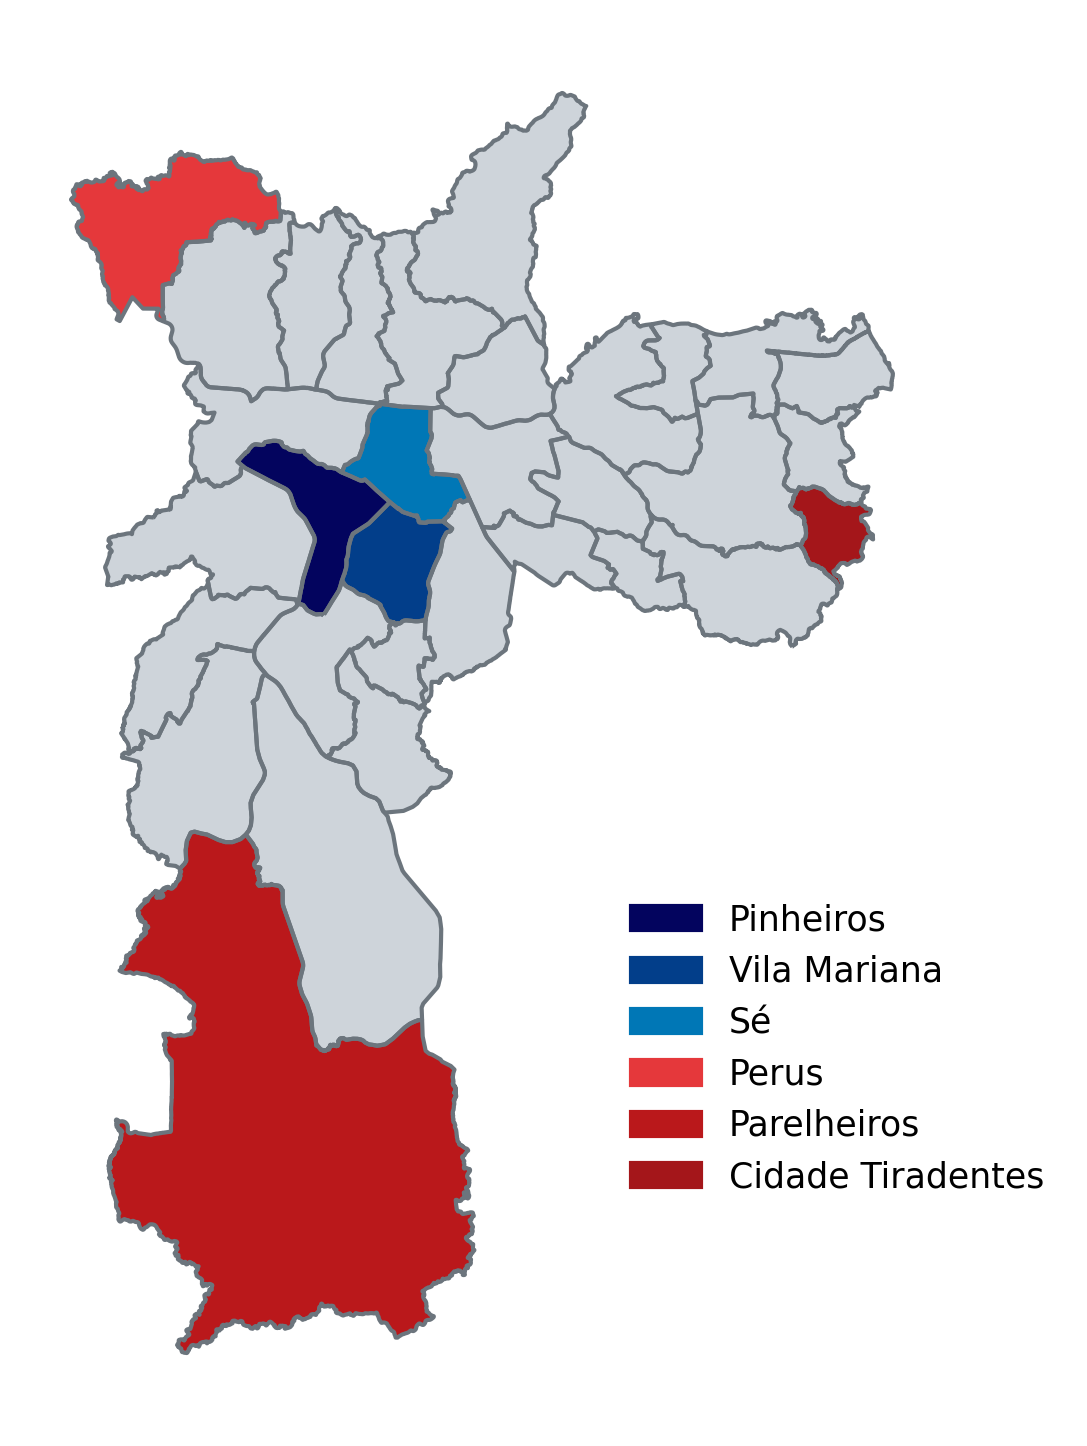
\includegraphics[width=\textwidth]{q1_a.png}
    \caption*{\emph{Total}}
  \end{subfigure}
  \hfill % This adds spacing between the subfigures
  \begin{subfigure}[b]{0.32\textwidth}
    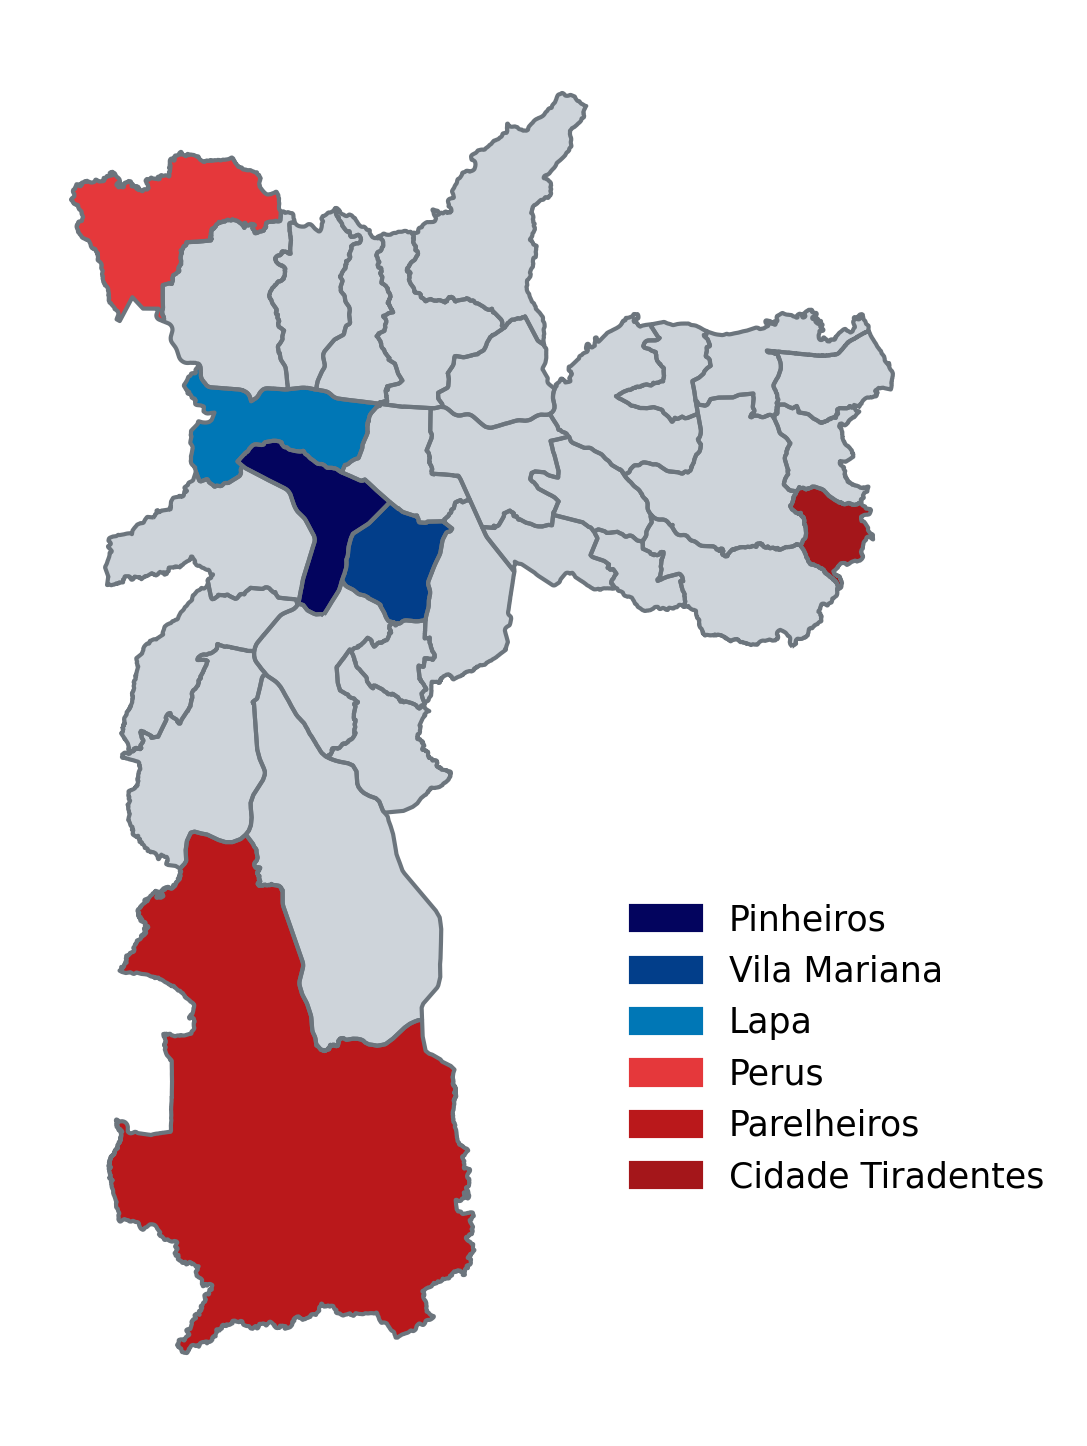
\includegraphics[width=\textwidth]{q1_b.png}
    \caption*{\emph{Residencial}}
  \end{subfigure}
  \hfill % This adds spacing between the subfigures
  \begin{subfigure}[b]{0.32\textwidth}
    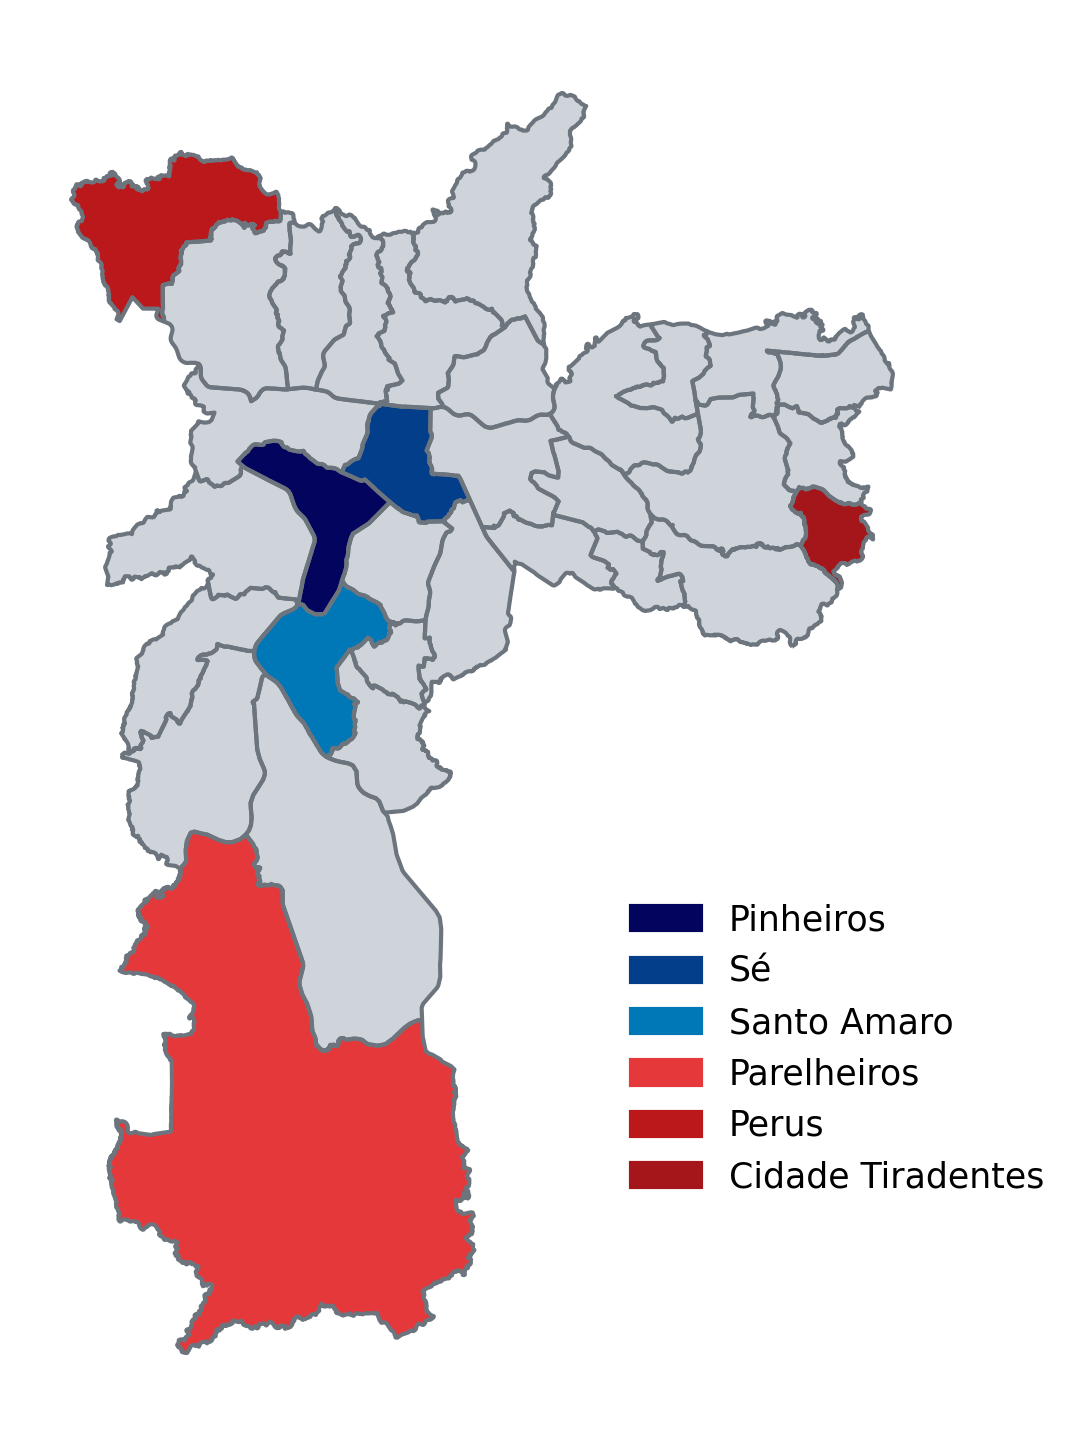
\includegraphics[width=\textwidth]{q1_c.png}
    \caption*{\emph{Demais Imóveis}}
  \end{subfigure}
\end{figure}

\ident Em conjuto, elas representaram 40\% dos 13.6 bilhões de reais arrecadaos em IPTU na cidade de São Paulo em 2023.\\

\textbf{Item 2}\\
\ident Em relação aos distritos, nota-se padrão semelhante: no centro estão os imóveis mais rentáveis, enquanto na periferia, os menos. Isso se deve, sobretudo, pelo fato do IPTU ser calculado sobre o valor venal, que considera o preço do $m^2$ no seu cálculo. Além disso, imóveis residenciais com valor venal abaixo de R\$ 230 mil não pagam IPTU, enquanto para os não residenciais, esse faixa é de R\$ 120 mil. Dado que muitos dos imóveis nas periferias ficam abaixo desse limiar, a arrecadção de IPTU nessas áreas é impactada.\\

\begin{figure}[htbp]
  \centering
  % Adjust the widths and the figure names to suit your document
  \begin{subfigure}[b]{0.32\textwidth}
    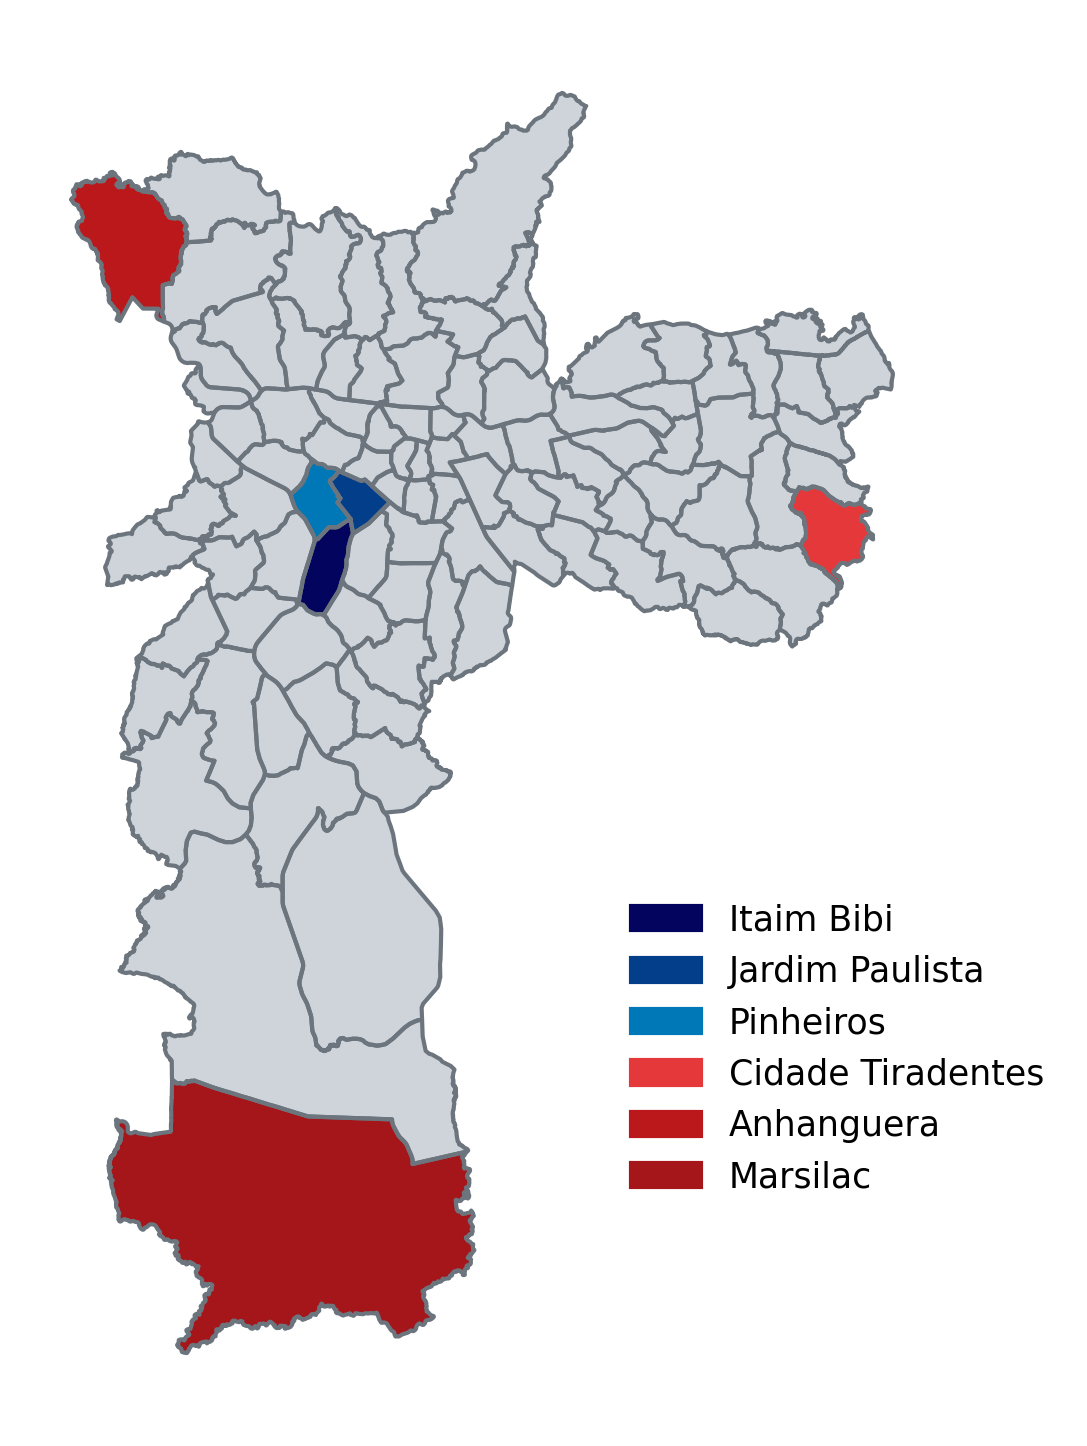
\includegraphics[width=\textwidth]{q2_a.png}
    \caption*{\emph{Total}}
  \end{subfigure}
  \hfill % This adds spacing between the subfigures
  \begin{subfigure}[b]{0.32\textwidth}
    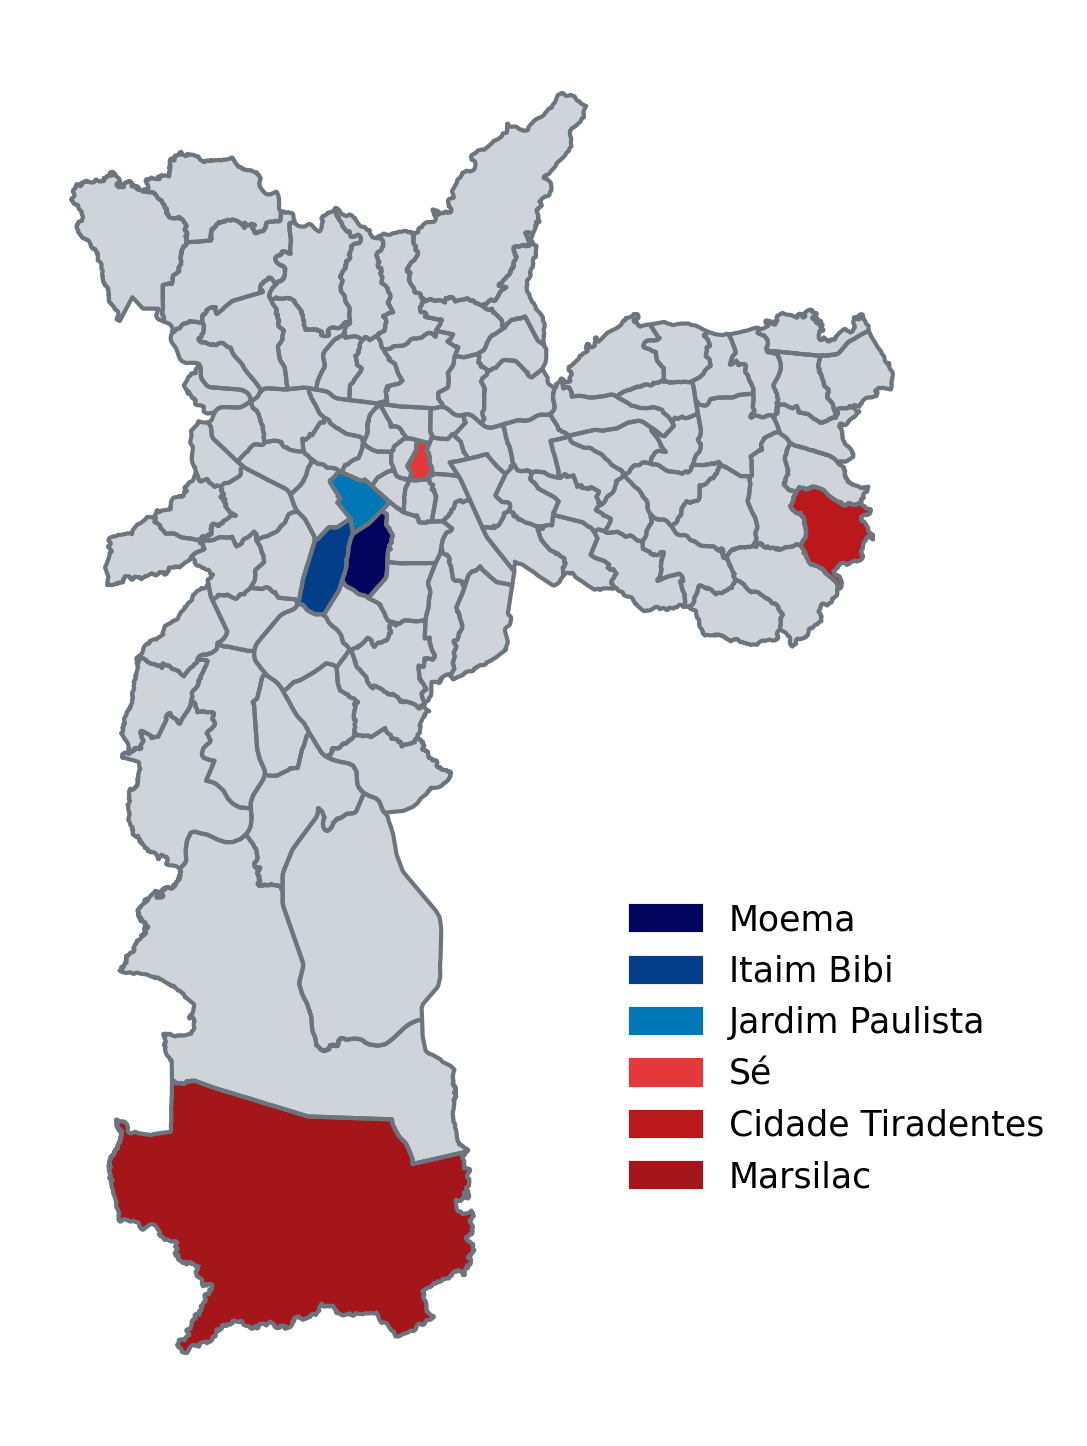
\includegraphics[width=\textwidth]{q2_b.png}
    \caption*{\emph{Residencial}}
  \end{subfigure}
  \hfill % This adds spacing between the subfigures
  \begin{subfigure}[b]{0.32\textwidth}
    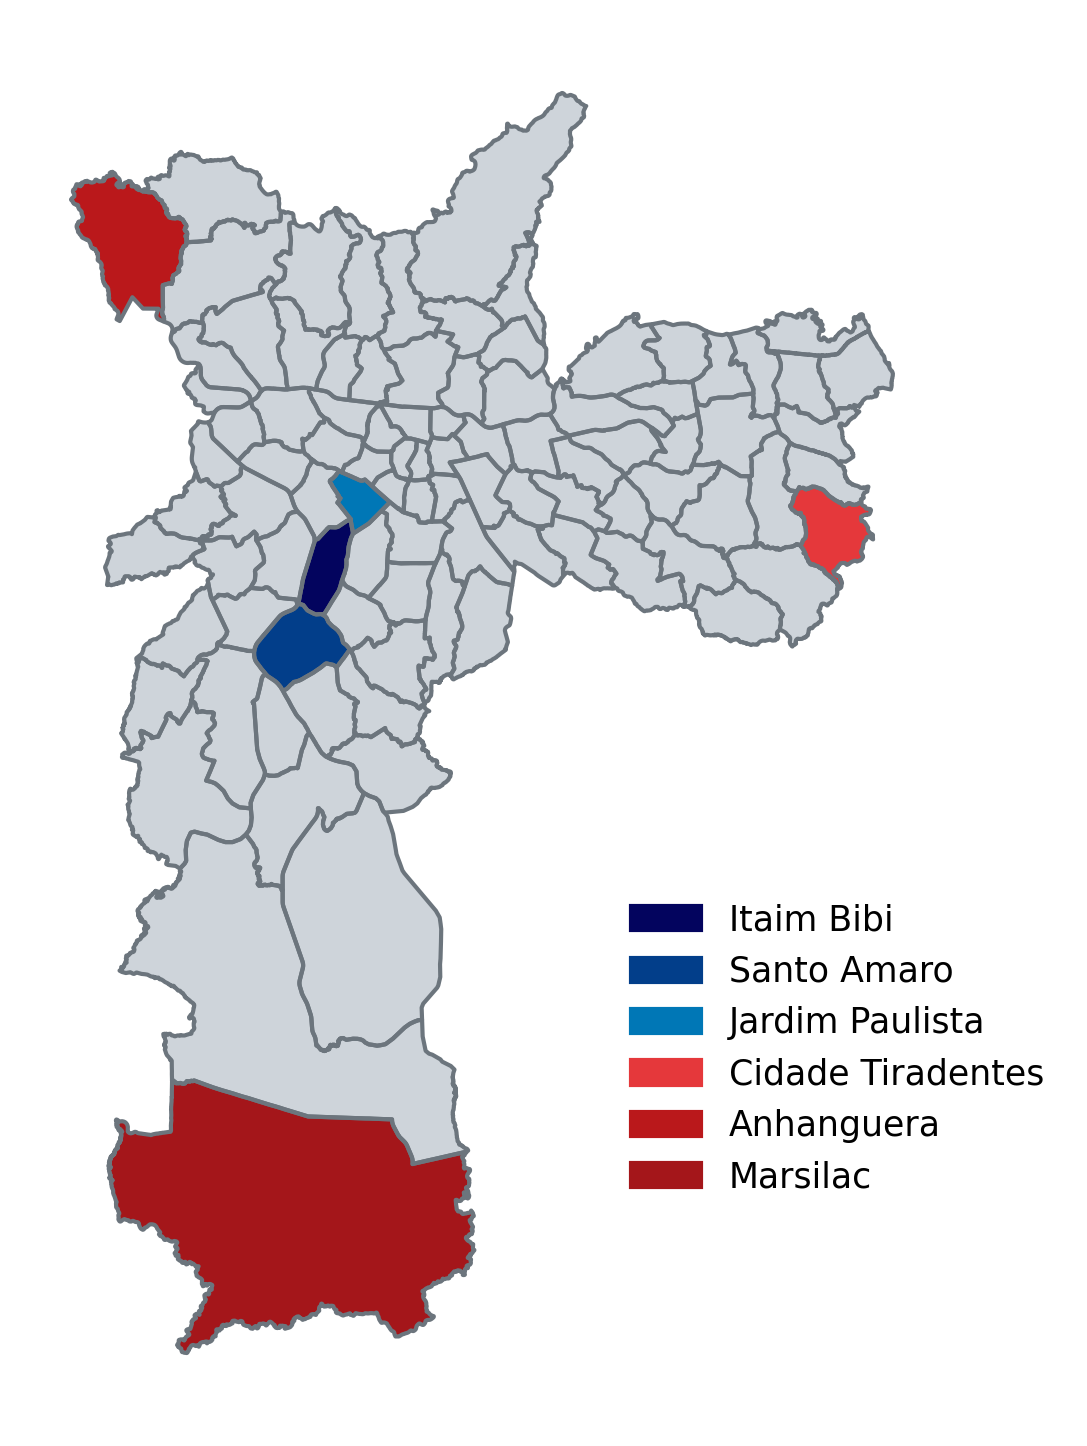
\includegraphics[width=\textwidth]{q2_c.png}
    \caption*{\emph{Demais Imóveis}}
  \end{subfigure}
\end{figure}

\textbf{Item 3}\\
\ident Por fim, as ruas que mais geram IPTU em São Paulo também estão no centro. Em 2023, a prefeitura arrecadou R\$ 242 milhões de reais em IPTU na Av. das Nações Unidas, mais do que qualquer outro endereço da cidade. Em segundo lugar está a Av. Brig. Faria Lima, seguidos da Av. Paulista, Av. Pres. Juscelino Kubitschek e Av. Escola Politécnica.\\

\begin{center}
    \includegraphics[width=0.8\textwidth]{top5_streets.png}
    \captionof{figure}{Logradouros que Mais Geraram IPTU em 2023}
\end{center}

\textbf{Extensões}\\
\ident Há inúmeros insights que podemos retirar dos dados. Alguns deles são:\\
\begin{itemize}
    \item O distrito de Itaim Bibi (e a subprefeitura de Pinheiros) sempre estão entre no top 3 dos que mais geram IPTU.
    \item Marsilac (e Parelheiros), por sua vez, sempre estão entre os que menos geram o imposto. São regiões pouco populosas e com \( m^2 \) barato, o que torna vários imóveis isentos de IPTU.
    \item Dado que temos o endereço de cada contribuinte, podemos saber quais imóveis mais pagam IPTU em São Paulo. Em primeiro lugar está, provavelmente, a USP. Em segundo, o Aeroporto de Congonhas. O terceiro parece ser o Parque Ibirapuera. Não sabemos o nome de cada estabelecimento, mas sabemos o endereço e a área do terreno de cada imóvel. Por isso, podemos inferir com precisão quais são os estabelecimentos que mais pagam IPTU na cidade. No código há um exemplo de como usar o \href{https://nominatim.org/release-docs/latest/api/Overview/}{Nominatim} para encontrar as coordenadas de um endereço.\\
    Os 10 imóveis que mais pagaram IPTU em 2023 foram:\\
\begin{center}
    \includegraphics[width=0.8\textwidth]{top10_imoveis.png}
    \captionof{figure}{Imóveis que Mais Geraram IPTU em 2023}
\end{center}
    \item O GeoSampa disponibiliza diversos outros datasets, com dados também delimitados por distrito. Podemos investigar se os distritos que mais pagam IPTU também são mais arborizados, têm mais iluminação urbana ou estão mais perto de uma estação de metrô, por exemplo.
    \item Dado que o IPTU é calculado sobre o valor venal, uma métrica cujo cálculo é determinado por lei, podemos simular como a arrecadação mudaria se a Prefeitura alterasse, marginalmente, as alíquotas e faixas de isenção.
\end{itemize}
\end{document}
